\documentclass[11pt,a4paper,openany]{report}

% ============================================================ Paquets
\usepackage[utf8]{inputenc}
\usepackage[T1]{fontenc}
\usepackage{mathpazo}                 % Palatino (texte + maths)
\usepackage[scaled=0.92]{helvet}      % Helvetica pour les titres
\linespread{1.06}
\IfFileExists{french.ldf}{\usepackage[english,french]{babel}}{\usepackage[english]{babel}}
\usepackage[a4paper,top=2.6cm,bottom=2.6cm,left=2.6cm,right=2.4cm,headheight=22pt]{geometry}
\usepackage{microtype}
\usepackage{amsmath,amssymb}
\usepackage{graphicx}
\usepackage{float}
\usepackage{booktabs,tabularx,multirow,array}
\usepackage[table]{xcolor}
\usepackage{tikz}
\usetikzlibrary{positioning,arrows.meta,calc,babel}
\usepackage{enumitem}
\usepackage[font=small,labelfont={bf,sf,color=primary},labelsep=period]{caption}
\usepackage{titlesec}
\usepackage{fancyhdr}
\usepackage[most]{tcolorbox}
\usepackage[hidelinks]{hyperref}

% ============================================================ Couleurs et styles
\definecolor{emsigreen}{HTML}{6AA84F}   % vert EMSI
\definecolor{primary}{HTML}{3E7A2B}     % vert foncé (titres, texte)
\definecolor{accent}{HTML}{6AA84F}
\definecolor{chartorange}{HTML}{F47230}
\definecolor{seriesblue}{HTML}{257DE0}
\definecolor{lightbg}{HTML}{F1F7EE}
\definecolor{rulegray}{HTML}{C8D9BF}
\definecolor{textgray}{HTML}{5A6270}

\setlist{itemsep=2pt,topsep=4pt,leftmargin=*}
\renewcommand{\arraystretch}{1.2}
\newcommand{\code}[1]{\texttt{\small #1}}
\newcommand{\best}[1]{\textbf{\color{primary}#1}}

% Titres de chapitres : numéro en couleur + filet
\titleformat{\chapter}[display]
  {\sffamily\bfseries\color{primary}}
  {\Large\color{accent}\MakeUppercase{\chaptertitlename}~\thechapter}
  {4pt}
  {\Huge}
  [\vspace{4pt}{\color{rulegray}\titlerule[1.2pt]}]
\titlespacing*{\chapter}{0pt}{-10pt}{22pt}
\titleformat{\section}{\sffamily\Large\bfseries\color{primary}}{\thesection}{0.8em}{}
\titleformat{\subsection}{\sffamily\large\bfseries\color{primary}}{\thesubsection}{0.8em}{}
\titlespacing*{\section}{0pt}{16pt}{6pt}

% En-têtes et pieds de page
\pagestyle{fancy}
\fancyhf{}
\renewcommand{\chaptermark}[1]{\markboth{#1}{}}
\fancyhead[L]{\sffamily\footnotesize\color{textgray}PRIORITEST-STAR}
\fancyhead[R]{\sffamily\footnotesize\color{textgray}\leftmark}
\fancyfoot[C]{\sffamily\small\color{textgray}\thepage}
\renewcommand{\headrulewidth}{0.4pt}
\renewcommand{\headrule}{\hbox to\headwidth{\color{rulegray}\leaders\hrule height \headrulewidth\hfill}}
\fancypagestyle{plain}{\fancyhf{}\fancyfoot[C]{\sffamily\small\color{textgray}\thepage}\renewcommand{\headrulewidth}{0pt}}

% Encadrés
\newtcolorbox{keybox}[1][À retenir]{enhanced,colback=lightbg,colframe=primary,boxrule=0pt,
  leftrule=3pt,arc=2pt,left=8pt,right=8pt,top=6pt,bottom=6pt,
  title={\sffamily\bfseries #1},coltitle=primary,colbacktitle=lightbg,attach title to upper={\par\smallskip}}
\newtcolorbox{warnbox}[1][Attention]{enhanced,colback=chartorange!6,colframe=chartorange,boxrule=0pt,
  leftrule=3pt,arc=2pt,left=8pt,right=8pt,top=6pt,bottom=6pt,
  title={\sffamily\bfseries #1},coltitle=chartorange!80!black,colbacktitle=chartorange!6,attach title to upper={\par\smallskip}}

% Libellés en français, même sans le module babel-french
\makeatletter
\newcommand{\setfrenchnames}{%
  \renewcommand{\chaptername}{Chapitre}\renewcommand{\contentsname}{Table des matières}%
  \renewcommand{\listfigurename}{Liste des figures}\renewcommand{\listtablename}{Liste des tableaux}%
  \renewcommand{\figurename}{Figure}\renewcommand{\tablename}{Tableau}\renewcommand{\bibname}{Références}}
\makeatother
\addto\captionsenglish{\setfrenchnames}\addto\captionsfrench{\setfrenchnames}\AtBeginDocument{\setfrenchnames}

% ============================================================ Document
\begin{document}

% ------------------------------------------------------------ Page de titre
\begin{titlepage}
\setlength{\parindent}{0pt}
\begin{tikzpicture}[remember picture,overlay]
  % barres vertes du style EMSI
  \fill[emsigreen] ([yshift=-1.3cm]current page.north west) rectangle ([xshift=12.6cm,yshift=-1.75cm]current page.north west);
  \node[anchor=north east,inner sep=0] at ([xshift=-2.4cm,yshift=-2.0cm]current page.north east)
       {
\includegraphics[width=6.2cm]{figures/emsi_logo.png}};
  \fill[emsigreen] ([xshift=7.4cm,yshift=-3.85cm]current page.north west) rectangle ([yshift=-4.3cm]current page.north east);
  % équerre à droite
  \fill[emsigreen] ([xshift=-5.2cm,yshift=-8.4cm]current page.north east) rectangle ([yshift=-8.85cm]current page.north east);
  \fill[emsigreen] ([xshift=-5.2cm,yshift=-8.4cm]current page.north east) rectangle ([xshift=-4.75cm,yshift=-10.2cm]current page.north east);
\end{tikzpicture}

\vspace*{3.6cm}
{\sffamily\bfseries\fontsize{26}{30}\selectfont PROJET CAPSTONE\par}
\vspace{0.3cm}
{\sffamily\bfseries\Large\hspace*{4.2cm}Année universitaire 2026--2027\par}

\vspace{2.6cm}
{\sffamily\bfseries\fontsize{30}{34}\selectfont\color{primary} PRIORITEST-STAR\par}
\vspace{0.35cm}
{\sffamily\large\color{textgray} Priorisation des classes logicielles à risque de défaut par représentations
spatio-temporelles, fusion guidée par similarité et apprentissage contrastif du classement\par}

\vspace{1.4cm}
{\sffamily\bfseries\fontsize{20}{24}\selectfont Ingénierie Informatique et Réseaux\par}
\vspace{0.15cm}
{\sffamily\large Option Data \& Intelligence Artificielle\par}
\vspace{0.25cm}
\noindent{\color{emsigreen}\rule{\linewidth}{1.6pt}\par}

\vspace{0.9cm}
\noindent\hspace*{0.3cm}{\color{emsigreen}\rule{5pt}{3.6cm}}\hspace{0.7cm}%
\begin{minipage}[b]{10cm}\sffamily\large
\textbf{Réalisé par :}\\[0.35cm]
\rule{0pt}{0pt}\\[0.5cm]

\rule{0pt}{0pt}\\[0.2cm]
\end{minipage}

\vfill
\end{titlepage}

\pagenumbering{roman}

% ------------------------------------------------------------ Résumé
\chapter*{Résumé}
\addcontentsline{toc}{chapter}{Résumé}
\markboth{Résumé}{}
Le budget de test étant limité, une équipe doit choisir quelles classes inspecter en priorité.
PRIORITEST-STAR classe les classes Java d'une version selon leur risque de contenir un défaut.
Chaque classe est décrite selon deux vues : une vue \emph{temporelle} (20 métriques orientées objet et de taille
sur trois versions successives, encodées par un réseau convolutif temporel causal) et une vue \emph{structurelle}
(le graphe des \code{import} Java explicites, encodé par un GraphSAGE compact à deux couches).
L'accord cosinus entre les deux vues guide leur fusion, et le modèle est entraîné avec une entropie croisée binaire,
une perte contrastive InfoNCE inter-vues et une perte de classement RankNet.

L'évaluation porte sur le projet Ant du jeu PROMISE, avec un protocole chronologique strict (entraînement sur la
version~1.5, validation sur~1.6, test unique sur~1.7), plusieurs graines aléatoires et des métriques sensibles à
l'effort. L'audit du pipeline fourni n'a révélé aucune fuite de labels, mais un très petit jeu d'entraînement et un
décalage de la proportion de classes défectueuses. Nous proposons donc \textbf{STAR-R}, une procédure d'entraînement
à variance réduite : recherche d'hyperparamètres sur la seule validation avec arrêt anticipé moyenné sur les graines,
ensemble de 10 graines, ré-entraînement sur entraînement et validation, et mélange avec deux modèles tabulaires
choisi sur la validation. Nous comparons ensuite tous les modèles avec le même budget de réglage sur la seule
validation, 10 graines, des intervalles de confiance par bootstrap et des tests appariés, puis étendons l'étude aux
projets Camel, POI et JEdit.

Sur la version de test d'Ant, jamais utilisée pour les réglages, STAR-R atteint une précision moyenne (AP) de
$0{,}799\pm0{,}003$, une accuracy de $0{,}823\pm0{,}004$ (classe majoritaire : $0{,}651$), un F1 de $0{,}745$ et un
MCC de $0{,}610$, contre $0{,}760\pm0{,}024$ d'AP et $0{,}751$ d'accuracy pour le modèle initial. À réglage égal,
cependant, aucun mécanisme de STAR n'apporte de gain significatif sur Ant : toutes les variantes font jeu égal avec une
régression logistique régularisée (AP $\approx0{,}80$, IC à 95\,\% d'environ $\pm0{,}07$). Le constat change sur
Camel, la plus grande version de test (565 classes) : réglé sur sa propre version d'entraînement, STAR avec le graphe
d'imports dépasse la régression logistique d'environ $+0{,}09$ d'AP ($p\le0{,}01$). Sur l'ensemble des projets,
STAR exploite mieux qu'un modèle linéaire les données d'autres projets, et la perte RankNet dégrade systématiquement
les résultats. Trier les classes par risque par ligne de code, plutôt que par risque brut, trouve 2,5 fois plus de
défauts pour un budget de 20\,\% du code sur Ant. Une application Streamlit permet d'explorer la liste priorisée.

\medskip\noindent\textbf{Mots-clés :} prédiction de défauts logiciels, priorisation des tests, réseau convolutif
temporel, GraphSAGE, apprentissage contrastif, apprentissage du classement, évaluation sensible à l'effort.

{\hypersetup{linkcolor=black}\tableofcontents}
\listoffigures
{\let\clearpage\relax\let\cleardoublepage\relax\vspace{1cm}\listoftables}

\cleardoublepage
\pagenumbering{arabic}

% ============================================================ 1. Objectif
\chapter{Objectif et fonctionnalités du projet}

\section{Contexte}
Un défaut découvert tard dans le cycle de développement coûte cher à corriger, et une équipe ne peut pas tester
toutes les classes d'un logiciel avec le même soin. La \emph{prédiction de défauts} vise à orienter l'effort de test
vers les classes les plus susceptibles d'être défectueuses. Pour une classe Java, deux sources d'information sont
disponibles : son \emph{historique} (l'évolution de ses métriques au fil des versions) et sa \emph{position dans
l'architecture} (les classes qu'elle utilise).

\section{Problématique}
La fiche du projet formule la question de recherche suivante :
\begin{keybox}[Question de recherche]
\itshape Une fusion guidée par la similarité temporelle--structurelle, renforcée par un alignement contrastif
inter-vues, améliore-t-elle le classement sensible à l'effort des classes défectueuses ?
\end{keybox}
Cette hypothèse doit être \emph{testée}, non présupposée : une réponse négative ou nuancée, obtenue avec un protocole
rigoureux, est un résultat valable.

\section{Objectifs}
\begin{enumerate}
  \item Produire, pour chaque classe d'une version, un \textbf{score de risque} et un \textbf{ordre d'inspection}.
  \item Exploiter conjointement l'historique des métriques (vue temporelle) et le graphe d'imports (vue structurelle).
  \item Évaluer sous \textbf{budget d'inspection} (20\,\% des classes, 20\,\% des lignes de code) et pas seulement
        en classification.
  \item Respecter un protocole sans fuite : réglages sur la validation uniquement, test utilisé une seule fois.
  \item Comparer à des références fortes et mesurer l'apport de chaque mécanisme par ablation.
  \item Fournir un outil de visualisation de la liste priorisée.
\end{enumerate}

\section{Définition précise de la tâche}
\begin{warnbox}[Précautions d'interprétation]
\begin{itemize}[leftmargin=1em]
  \item Le label indique si la classe contient au moins un défaut \emph{dans la version cible}, et les métriques
        de cette version font partie de l'entrée : c'est une \textbf{détection des défauts de la version observée},
        pas une prédiction de la version suivante.
  \item Le graphe ne contient que les \code{import} Java explicitement détectés : c'est un graphe de dépendances
        \textbf{partiel}.
\end{itemize}
\end{warnbox}

\section{Fonctionnalités livrées}
\begin{table}[htbp]
\centering\small
\caption{Scripts et fonctionnalités du dépôt \code{KIT\_MULTI\_PROJETS}.}
\label{tab:scripts}
\begin{tabularx}{\linewidth}{>{\raggedright\arraybackslash}p{4.4cm}X}
\toprule
\textbf{Fichier} & \textbf{Rôle} \\
\midrule
\code{prepare\_multi.py} & Construit les fenêtres de trois versions à partir de l'archive PROMISE (fourni). \\
\code{check\_graph\_temporal.py}\newline\code{tests/} & Contrôle des données et 36 tests unitaires (modèle, métriques,
statistiques, absence de fuite vers le test). \\
\code{src/model.py} & Modèle CrossViewSTAR (TCN, GraphSAGE, fusion, têtes) et pertes InfoNCE / RankNet. \\
\code{src/train.py} & Chargement des données et métriques d'évaluation. \\
\code{src/stats.py} & \emph{Ajouté.} $P_{\mathrm{opt}}$, IFA, intervalles de confiance par bootstrap, tests appariés,
Wilcoxon, delta de Cliff, Scott-Knott ESD. \\
\code{run\_star.py} & Ablations A1--A8 sur plusieurs graines (référence de départ). \\
\code{explore\_val.py} & \emph{Ajouté.} Recherche de 192 configurations $\times$ 3 graines sur la validation seule. \\
\code{train\_final.py} & \emph{Ajouté.} Entraînement final STAR-R, choix sur validation, test évalué une fois, 5 répétitions. \\
\code{analyse\_star.py} & \emph{Ajouté.} Courbe effort--rappel, poids de fusion, erreurs typiques, liste priorisée. \\
\code{app.py} & \emph{Ajouté.} Application Streamlit de visualisation du Top-$k$. \\
\code{compare\_fair.py} & \emph{Ajouté.} Comparaison à réglage égal de A1--A7 et des références, avec tests (sec.~\ref{sec:fair}). \\
\code{effort\_star.py}, \code{more\_data.py},\newline\code{improve\_star.py} & \emph{Ajoutés.} Effort appris dans le
modèle, données d'autres projets, améliorations de la fusion et du contraste (sec.~\ref{sec:effort}--\ref{sec:improve}). \\
\code{transfer\_study.py},\newline\code{retune\_project.py} & \emph{Ajoutés.} Généralisation à Camel, POI et JEdit,
avec réglages figés ou réglage interne (sec.~\ref{sec:transfer}). \\
\code{graph\_analysis.py} & \emph{Ajouté.} Statistiques des graphes et apport du graphe selon le degré (sec.~\ref{sec:graph}). \\
\bottomrule
\end{tabularx}
\end{table}

\noindent Les commandes complètes de reproduction sont données à la section~\ref{sec:repro}.

% ============================================================ 2. État de l'art
\chapter{État de l'art}

\section{Métriques logicielles et prédiction de défauts}
La suite de Chidamber et Kemerer~\cite{ck1994} (WMC, DIT, NOC, CBO, RFC, LCOM) est la base des métriques orientées
objet. Basili et al.~\cite{basili1996} ont montré empiriquement que plusieurs de ces métriques sont associées à la
propension aux fautes. Jureczko et Madeyski~\cite{jureczko2010} ont publié des jeux de métriques étendues (Ca, Ce,
NPM, LCOM3, LOC, DAM, MOA, MFA, CAM, IC, CBM, AMC, Max/Avg CC) pour de nombreux projets Java open source : ce sont
les 20 métriques du dépôt PROMISE utilisées ici.

Les premiers travaux appliquent des classifieurs classiques à ces attributs~\cite{menzies2007}.
Lessmann et al.~\cite{lessmann2008} comparent 22 classifieurs et observent que les écarts entre les meilleurs sont
souvent faibles ; Ghotra et al.~\cite{ghotra2015} nuancent ce constat et montrent que le choix de la technique peut
compter. Tantithamthavorn et al.~\cite{tantithamthavorn2016} soulignent que le réglage des hyperparamètres modifie
sensiblement les performances, ce qui impose de régler toutes les méthodes avec le même soin. Enfin, les métriques de
\emph{changement} entre versions sont souvent plus informatives que les seules métriques statiques~\cite{moser2008},
ce qui motive l'usage de l'historique et des variations $\Delta x$.

\section{Apprentissage profond}
Wang et al.~\cite{wang2016} apprennent des caractéristiques sémantiques à partir des arbres syntaxiques par un réseau
de croyance profond, et Li et al.~\cite{li2017} utilisent un réseau convolutif sur les jetons du code.
Sur des métriques tabulaires, Rhazi et al.~\cite{rhazi2026} proposent un apprentissage contrastif de la similarité
entre classes, avec attention inter-échantillons et similarité cosinus de Frobenius, et rapportent de meilleurs F1
que Random Forest, XGBoost, CatBoost, FT-Transformer et SAINT sur neuf projets (PROMISE, AEEEM, ReLink).
Leur évaluation repose sur un découpage aléatoire au sein d'une même version, un F1 pondéré par la fréquence des
classes et une prédiction par vote des $N$ classes d'entraînement les plus similaires, sans métrique sensible à
l'effort : nos résultats, obtenus avec un protocole chronologique, ne sont donc pas directement comparables aux leurs.
PRIORITEST-STAR reprend le \emph{principe} d'apprentissage des similarités mais pas leur architecture : ici, la
similarité relie deux vues d'une \emph{même} classe et sert à guider leur fusion.

\section{Graphes de dépendances}
Zimmermann et Nagappan~\cite{zimmermann2008} montrent que des mesures de réseau calculées sur le graphe de
dépendances améliorent la prédiction de défauts. Les réseaux de neurones sur graphes généralisent cette idée :
GraphSAGE~\cite{hamilton2017} apprend la représentation d'un nœud en agrégeant celles de ses voisins, de façon
inductive.

\section{Modélisation temporelle}
Les réseaux convolutifs temporels (TCN)~\cite{bai2018} utilisent des convolutions causales et dilatées : la sortie à
l'instant $t$ ne dépend que des entrées antérieures ou égales à $t$. Ils sont une alternative simple et stable aux
réseaux récurrents pour de courtes séquences, comme nos trois versions.

\section{Apprentissage contrastif et classement}
InfoNCE~\cite{oord2018} apprend des représentations en rapprochant une paire positive et en éloignant des négatifs.
SimCLR~\cite{chen2020} l'a popularisé avec des vues augmentées d'une même image, et sa version
supervisée~\cite{khosla2020} utilise les labels pour ne pas traiter comme négatifs des exemples de même classe (faux
négatifs). RankNet~\cite{burges2005} apprend un ordre en optimisant une perte logistique sur des paires d'exemples.

\section{Évaluation sensible à l'effort}
Inspecter une grande classe coûte plus cher qu'en inspecter une petite. Mende et Koschke~\cite{mende2010} et Kamei
et al.~\cite{kamei2013} proposent d'évaluer et de trier les classes en tenant compte de ce coût, mesuré en lignes de
code. Yang et al.~\cite{yang2016} montrent que des modèles très simples peuvent être compétitifs dans ce cadre :
une référence simple et bien réglée est donc indispensable.

\section{Positionnement}
\begin{keybox}[Positionnement de PRIORITEST-STAR]
À notre connaissance, aucune des approches ci-dessus ne combine dans un même modèle (i) l'historique des métriques
par TCN, (ii) le graphe d'imports par GraphSAGE, (iii) une fusion pondérée par l'accord cosinus entre ces deux vues,
et (iv) un alignement contrastif inter-vues avec une tête de classement. La contribution est aussi méthodologique :
protocole chronologique strict, ablations à un seul mécanisme et mesure explicite de la variance.
\end{keybox}

% ============================================================ 3. Architecture
\chapter{Architecture du modèle}

\section{Vue d'ensemble}
La figure~\ref{fig:archi} résume le modèle. Pour chaque classe $i$, deux encodeurs produisent un vecteur temporel
$z_T^{(i)}$ et un vecteur structurel $z_S^{(i)}$ de dimension $d=32$. Leur accord cosinus guide une fusion apprise,
suivie de deux têtes : une tête de risque et une tête de classement.

\begin{figure}[htbp]
\centering
\resizebox{\linewidth}{!}{%
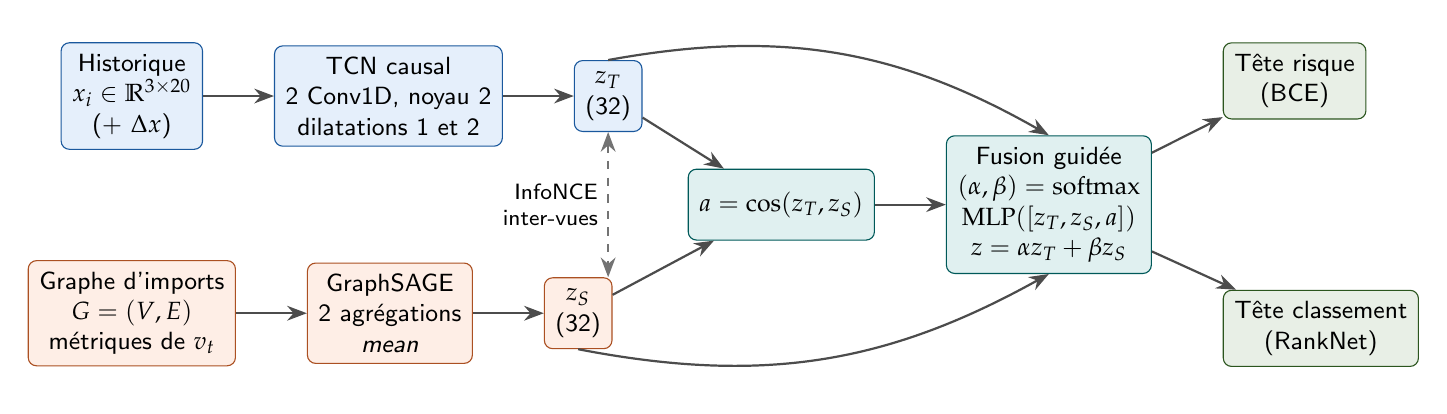
\begin{tikzpicture}[
  node distance=6mm and 9mm,
  box/.style={draw=#1!70!black, rounded corners=3pt, align=center, minimum height=9mm, inner sep=4pt,
              fill=#1!12, font=\sffamily\small},
  arr/.style={-{Stealth[length=2.5mm]}, thick, color=black!70}]
  \node[box=seriesblue] (hist) {Historique\\ $x_i\in\mathbb{R}^{3\times20}$\\ (+ $\Delta x$)};
  \node[box=seriesblue, right=of hist] (tcn) {TCN causal\\ 2 Conv1D, noyau 2\\ dilatations 1 et 2};
  \node[box=seriesblue, right=of tcn] (zt) {$z_T$\\ (32)};
  \node[box=chartorange, below=14mm of hist] (graph) {Graphe d'imports\\ $G=(V,E)$\\ métriques de $v_t$};
  \node[box=chartorange, right=of graph] (sage) {GraphSAGE\\ 2 agrégations\\ \textit{mean}};
  \node[box=chartorange, right=of sage] (zs) {$z_S$\\ (32)};
  \node[box=teal, right=12mm of $(zt)!0.5!(zs)$] (cos) {$a=\cos(z_T,z_S)$};
  \node[box=teal, right=of cos] (gate) {Fusion guidée\\ $(\alpha,\beta)=\mathrm{softmax}$\\ $\mathrm{MLP}([z_T,z_S,a])$\\ $z=\alpha z_T+\beta z_S$};
  \node[box=primary, above right=2mm and 9mm of gate] (risk) {Tête risque\\ (BCE)};
  \node[box=primary, below right=2mm and 9mm of gate] (rank) {Tête classement\\ (RankNet)};
  \draw[arr] (hist) -- (tcn); \draw[arr] (tcn) -- (zt);
  \draw[arr] (graph) -- (sage); \draw[arr] (sage) -- (zs);
  \draw[arr] (zt) -- (cos); \draw[arr] (zs) -- (cos);
  \draw[arr] (cos) -- (gate);
  \draw[arr] (zt.north) to[bend left=20] (gate.north);
  \draw[arr] (zs.south) to[bend right=20] (gate.south);
  \draw[arr] (gate) -- (risk); \draw[arr] (gate) -- (rank);
  \draw[{Stealth[length=2.5mm]}-{Stealth[length=2.5mm]}, thick, dashed, black!55] (zt.south) --
     node[left, font=\sffamily\footnotesize, align=right, text=black]{InfoNCE\\inter-vues} (zt.south |- zs.north);
\end{tikzpicture}}
\caption{Architecture de PRIORITEST-STAR. La flèche pointillée indique la perte contrastive InfoNCE, appliquée
uniquement pendant l'entraînement.}
\label{fig:archi}
\end{figure}

\section{Vue temporelle : TCN causal}
L'entrée $x_i\in\mathbb{R}^{3\times F}$ ($F=20$ métriques, 3 versions) passe dans deux convolutions 1D causales de
noyau 2, de dilatations 1 puis 2, à 32 canaux et activation ReLU. Le rembourrage est retiré à droite : la sortie à la
version $t$ ne voit que les versions $\le t$. Le vecteur de la dernière version est projeté linéairement en
$z_T\in\mathbb{R}^{32}$. Dans STAR-R, l'entrée est enrichie des variations $\Delta x_t=x_t-x_{t-1}$ (avec
$\Delta x_0=0$), soit 40 canaux d'entrée.

\section{Vue structurelle : GraphSAGE compact}
Les métriques de la version cible passent par une couche linéaire suivie de ReLU, puis par deux couches d'agrégation
\emph{mean} :
\[
h_i^{(l+1)}=\mathrm{ReLU}\!\left(W_s^{(l)}h_i^{(l)}+W_n^{(l)}\,\frac{1}{|\mathcal{N}(i)|}\sum_{j\in\mathcal{N}(i)}h_j^{(l)}\right),
\]
où $\mathcal{N}(i)$ est l'ensemble des classes importées par $i$. C'est une version simplifiée de
GraphSAGE~\cite{hamilton2017} : l'agrégation porte sur tout le graphe de la version, sans échantillonnage de voisins.
Une projection donne $z_S\in\mathbb{R}^{32}$. Une variante bidirectionnelle agrège séparément les classes importées et
les classes qui importent.

\section{Fusion guidée par similarité}
L'accord entre les vues est $a_i=\cos\big(z_T^{(i)},z_S^{(i)}\big)$. Un MLP ($65\to32\to2$) suivi d'un softmax
produit les poids $(\alpha_i,\beta_i)$, avec $\alpha_i+\beta_i=1$, et la représentation fusionnée est
$z_i=\alpha_i z_T^{(i)}+\beta_i z_S^{(i)}$. La variante « fusion classique » retire $a_i$ de l'entrée du MLP.
Les poids $\alpha,\beta$ et l'accord $a$ sont exportés pour chaque classe afin d'analyser quelle vue le modèle utilise
(section~\ref{sec:fusion}).

\section{Têtes et fonction de perte}
Deux têtes linéaires produisent un logit de risque $r_i$ et un score de classement $s_i$. La perte totale est
\[
\mathcal{L}=\mathcal{L}_{\mathrm{BCE}}(r,y)+\lambda_c\,\mathcal{L}_{\mathrm{InfoNCE}}(z_T,z_S)+\lambda_r\,\mathcal{L}_{\mathrm{RankNet}}(s,y).
\]
\begin{itemize}
  \item $\mathcal{L}_{\mathrm{BCE}}$ : entropie croisée binaire, pondérée par $w_+=N_-/N_+$ dans STAR-R pour compenser
        le déséquilibre des classes.
  \item $\mathcal{L}_{\mathrm{InfoNCE}}$ : InfoNCE symétrique de température $\tau$. La paire positive est
        $\big(z_T^{(i)},z_S^{(i)}\big)$ ; les négatifs sont les autres classes de la même version. Limite connue : deux
        classes défectueuses différentes peuvent devenir de faux négatifs (une variante masque ces paires).
  \item $\mathcal{L}_{\mathrm{RankNet}}=\frac{1}{|\mathcal{P}|}\sum_{(i,j)\in\mathcal{P}}\log\!\big(1+e^{-(s_i-s_j)}\big)$,
        sur des paires (défectueuse $i$, saine $j$) de la même version, au plus 3\,000 paires.
\end{itemize}
Le score de priorité utilisé pour l'évaluation est $\sigma(s_i)$ si $\lambda_r>0$, sinon $\sigma(r_i)$.
Le modèle compte 12\,644 paramètres (13\,924 avec l'entrée $\Delta x$) et s'entraîne par lot complet, une version
formant un lot, avec l'optimiseur Adam.

\section{Ablations A1--A8}
\begin{table}[htbp]
\centering\small
\caption{Configurations d'ablation : chacune ajoute un seul mécanisme à la précédente.}
\label{tab:ablations-def}
\begin{tabularx}{\linewidth}{@{}lX@{}}
\toprule
\textbf{Id} & \textbf{Configuration} \\
\midrule
A1 & Boosting (HistGradientBoosting) sur les métriques de la version cible \\
A2 & TCN seul + BCE (apport de l'historique seul) \\
A3 & + vue structurelle, fusion classique \\
A4 & + fusion guidée par l'accord cosinus \\
A5 & + InfoNCE inter-vues \\
A6 & + RankNet = STAR complet \\
A7 & STAR+ : $\Delta x$, GraphSAGE bidirectionnel, InfoNCE sans faux négatifs, RankNet pondéré par LOC, dropout + LayerNorm \\
A8 & Ensemble par moyenne des rangs de A1, A5 et A6 \\
\bottomrule
\end{tabularx}
\end{table}

\section{Procédure d'entraînement STAR-R}
\label{sec:starr}
Avec 118 classes d'entraînement, le principal problème est la \emph{variance} : l'AP de test de A6 varie de
$\pm0{,}024$ selon la graine, et l'époque retenue par l'arrêt anticipé varie de 10 à 48. STAR-R conserve
l'architecture et modifie la procédure d'entraînement :
\begin{enumerate}
  \item \textbf{Prétraitement} : compression $\mathrm{sign}(x)\log(1+|x|)$ des métriques standardisées, BCE pondérée,
        puis ré-entraînement final sur entraînement + validation.
  \item \textbf{Recherche sur la validation uniquement} : 192 configurations (taux d'apprentissage, weight decay,
        dropout, $\lambda_c$, $\lambda_r$, agrégation bidirectionnelle, $\Delta x$) $\times$ 3 graines, sans charger le
        test. Configuration retenue : taux d'apprentissage $10^{-3}$, weight decay $10^{-3}$, $\lambda_c=0{,}1$,
        $\lambda_r=0{,}25$, $\tau=0{,}2$, $\Delta x$ activé, sans dropout, agrégation unidirectionnelle.
  \item \textbf{Arrêt anticipé robuste} : l'époque (64) est choisie sur la courbe d'AP de validation \emph{moyennée sur
        les graines et lissée}, au lieu du maximum bruité de chaque graine.
  \item \textbf{Ensemble de 10 graines} : moyenne des rangs des scores.
  \item \textbf{Mélange choisi sur la validation} : régression logistique ($C=0{,}03$, classes équilibrées) et
        ExtraTrees (500 arbres) sur les métriques de la version cible et leurs variations. Le mélange (STAR seul, STAR+LR,
        STAR+ET, STAR+LR+ET) est choisi par l'AP de validation de modèles entraînés sur la version~1.5 seulement.
  \item \textbf{Seuil de décision} : fraction de classes signalées qui maximise l'accuracy de validation.
  \item \textbf{Répétition} : toute la procédure est répétée sur 5 groupes de graines indépendants.
\end{enumerate}

% ============================================================ 4. Données
\chapter{Données}

\section{Source}
Les données proviennent du dépôt PROMISE~\cite{jureczko2010}. Pour chaque version d'un projet Java, un fichier CSV
donne 20 métriques par classe et son nombre de défauts ; le code source permet d'extraire les \code{import}.

\section{Construction des fenêtres}
Le script \code{prepare\_multi.py} construit, pour chaque version cible $v_t$, une \textbf{fenêtre stricte} de trois
versions $(v_{t-2},v_{t-1},v_t)$ :
\begin{itemize}
  \item \textbf{Classes retenues} : seulement celles présentes dans les trois versions. Les classes nouvelles sont
        exclues, ce qui crée un biais de sélection et une couverture partielle (colonne « couv. » du
        tableau~\ref{tab:data}).
  \item \textbf{Entrée temporelle} $X\in\mathbb{R}^{N\times 3\times 20}$ : les 20 métriques de chaque classe aux trois
        versions.
  \item \textbf{Label} : $y_i=1$ si la classe a au moins un défaut dans $v_t$.
  \item \textbf{Graphe} : arête orientée $(i,j)$ si la classe $i$ contient \code{import j;} dans $v_t$ (imports
        statiques et génériques \code{.*} ignorés).
  \item \textbf{Coût} : nombre de lignes de code (LOC) de la classe dans $v_t$, utilisé comme approximation de l'effort
        d'inspection.
  \item \textbf{Normalisation} : centrage-réduction ajusté \emph{uniquement} sur la première fenêtre (entraînement) de
        chaque projet, puis écrêtage à $\pm10$.
\end{itemize}

\section{Statistiques}
\begin{table}[htbp]
\centering\small
\caption{Fenêtres préparées par projet. $N$ : classes ; $P$ : classes défectueuses ; $E$ : arêtes d'import ;
couv. : part des classes étiquetées de la version cible conservées.}
\label{tab:data}
\rowcolors{2}{}{lightbg}
\begin{tabular}{llrrrrr}
\toprule
\textbf{Projet} & \textbf{Cible (fenêtre)} & $\boldsymbol{N}$ & $\boldsymbol{P}$ & \textbf{\% déf.} & $\boldsymbol{E}$ & \textbf{couv.} \\
\midrule
Ant      & 1.5 (1.3--1.5) & 118 & 20  & 16,9 & 255  & 0,40 \\
Ant      & 1.6 (1.4--1.6) & 167 & 60  & 35,9 & 469  & 0,48 \\
Ant      & 1.7 (1.5--1.7) & 292 & 102 & 34,9 & 873  & 0,39 \\
JEdit    & 4.1 (3.2--4.1) & 253 & 61  & 24,1 & 157  & 0,81 \\
JEdit    & 4.2 (4.0--4.2) & 272 & 39  & 14,3 & 156  & 0,74 \\
JEdit    & 4.3 (4.1--4.3) & 179 & 5   & 2,8  & 236  & 0,36 \\
Camel    & 1.4 (1.0--1.4) & 252 & 57  & 22,6 & 646  & 0,29 \\
Camel    & 1.6 (1.2--1.6) & 565 & 127 & 22,5 & 1624 & 0,59 \\
POI      & 2.5 (1.5--2.5) & 224 & 153 & 68,3 & 294  & 0,58 \\
POI      & 3.0 (2.0--3.0) & 311 & 202 & 65,0 & 473  & 0,70 \\
Xalan    & 2.6 (2.4--2.6) & 655 & 268 & 40,9 & 2276 & 0,74 \\
Log4j    & 1.2 (1.0--1.2) & 93  & 86  & 92,5 & 149  & 0,45 \\
Lucene   & 2.4 (2.0--2.4) & 180 & 130 & 72,2 & 262  & 0,53 \\
Synapse  & 1.2 (1.0--1.2) & 149 & 50  & 33,6 & 403  & 0,58 \\
Velocity & 1.6 (1.4--1.6) & 152 & 50  & 32,9 & 508  & 0,66 \\
Xerces   & 1.3 (init--1.3)& 114 & 33  & 28,9 & 182  & 0,25 \\
\bottomrule
\end{tabular}
\end{table}

Ivy (aucune classe commune aux trois versions) et PBeans (deux versions seulement) ne sont pas préparés.

\section{Partitions et choix du projet d'étude}
Seuls Ant et JEdit disposent de trois fenêtres, donc d'une partition chronologique entraînement / validation / test.
\textbf{Ant est le projet principal} : entraînement sur 1.5, validation sur 1.6, test sur 1.7.
JEdit est écarté des conclusions : sa version de test 4.3 ne contient que 5 classes défectueuses sur 179, ce qui rend
les métriques instables (tous les modèles y obtiennent une accuracy inférieure à celle de la classe majoritaire,
0,972, et l'intervalle de confiance de l'AP couvre 0,05--0,70). Camel (1.4$\to$1.6) et POI (2.5$\to$3.0) n'ont pas de
validation indépendante : ils servent à tester la généralisation des conclusions (section~\ref{sec:transfer}), avec
les réglages figés depuis Ant ou avec un réglage interne à leur version d'entraînement. Les projets à une seule
fenêtre ne permettent pas de test chronologique interne ; ils servent seulement de données sources dans l'étude
inter-projets (section~\ref{sec:moredata}).

\section{Audit des données}
\begin{keybox}[Résultats de l'audit]
\begin{itemize}[leftmargin=1em]
  \item \textbf{Fuite de labels : aucune.} Les labels de test ne servent ni à l'entraînement, ni à l'arrêt anticipé,
        ni aux réglages, ni au choix du seuil ; aucune valeur manquante après préparation.
  \item \textbf{Recouvrement d'entités.} 117 des 118 classes d'entraînement et les 167 classes de validation
        réapparaissent dans la fenêtre de test (versions ultérieures des mêmes classes). Ce n'est pas une fuite de
        labels, mais le test ne porte pas sur du code inédit.
  \item \textbf{Déséquilibre et décalage de prévalence.} 17\,\% de classes défectueuses à l'entraînement contre 35\,\%
        en validation et en test. L'accuracy doit être comparée à la classe majoritaire (0,651 sur le test).
  \item \textbf{Queues lourdes.} LOC, RFC et WMC sont très asymétriques ; certaines valeurs atteignent l'écrêtage à $+10$.
  \item \textbf{Coûts quasi nuls.} 11 classes de test (des interfaces, aucune défectueuse) ont au plus 1 ligne de code.
        Elles ne pèsent rien dans un budget en LOC mais occupent des places dans un Top-$k$ en nombre de classes.
  \item \textbf{Petite taille.} 118 classes et 20 positifs à l'entraînement, d'où une forte variance entre graines.
\end{itemize}
\end{keybox}

% ============================================================ 5. Résultats
\chapter{Expérimentations et résultats}

\section{Protocole et métriques}
Ant : entraînement sur 1.5, validation sur 1.6, test sur 1.7, évalué une seule fois par répétition.
\begin{itemize}
  \item \textbf{Métriques principales} : précision moyenne (AP) de la classe défectueuse ; Recall@20\,\% des classes ;
        Recall@20\,\% LOC (budget strict, tri par risque) ; EA-Recall@20\,\% LOC (tri par densité score/LOC).
  \item \textbf{Métriques complémentaires} : ROC-AUC, accuracy, précision, rappel, F1, MCC, avec un seuil choisi sur
        la validation ; $P_{\mathrm{opt}}$, l'aire normalisée sous la courbe effort--rappel (1 = oracle, 0,5 $\approx$
        hasard).
  \item \textbf{Statistiques} (sections~\ref{sec:fair} et suivantes) : moyenne $\pm$ écart-type sur 10 graines,
        intervalle de confiance à 95\,\% par bootstrap sur les classes du test (2\,000 tirages)~\cite{efron1993},
        bootstrap apparié pour comparer deux modèles sur les mêmes classes, test de Wilcoxon~\cite{wilcoxon1945} sur
        les graines et delta de Cliff~\cite{romano2006} comme taille d'effet.
  \item \textbf{Environnement} : CPU (2 cœurs), PyTorch 2.15, scikit-learn 1.9, sans GPU. STAR-R a été réexécuté dans
        un second environnement (Linux) : AP de 0,798 sur la première répétition, contre $0{,}799\pm0{,}003$ en
        moyenne sur les cinq.
\end{itemize}

\section{Ablations avec la configuration d'origine}
\begin{table}[htbp]
\centering\small
\caption{Ant 1.7 (test), moyenne sur 5 graines (écart-type de l'AP), hyperparamètres par défaut du kit.}
\label{tab:abl}
\rowcolors{2}{}{lightbg}
\begin{tabular}{lcccccc}
\toprule
\textbf{Variante} & \textbf{AP} & \textbf{ROC-AUC} & \textbf{R@20\%cl.} & \textbf{EA-R@20\%LOC} & \textbf{Accuracy} & \textbf{MCC} \\
\midrule
A1 Boosting        & 0,753            & 0,843 & 0,461 & 0,314 & 0,771 & 0,472 \\
A2 TCN + BCE       & 0,718 $\pm$ 0,018 & 0,816 & 0,433 & 0,280 & 0,758 & 0,451 \\
A3 + graphe        & 0,716 $\pm$ 0,020 & 0,809 & 0,433 & 0,280 & 0,747 & 0,432 \\
A4 + fusion cos.   & 0,722 $\pm$ 0,016 & 0,810 & 0,445 & 0,284 & 0,756 & 0,455 \\
A5 + InfoNCE       & 0,743 $\pm$ 0,023 & 0,826 & 0,455 & 0,288 & 0,764 & 0,482 \\
A6 STAR complet    & 0,760 $\pm$ 0,024 & 0,832 & 0,467 & 0,312 & 0,751 & 0,480 \\
A7 STAR+           & 0,678 $\pm$ 0,042 & 0,765 & 0,422 & 0,310 & 0,745 & 0,414 \\
A8 Ensemble        & 0,797 $\pm$ 0,013 & 0,865 & 0,500 & 0,316 & 0,801 & 0,554 \\
\bottomrule
\end{tabular}
\end{table}

À partir de A4, chaque mécanisme ajoute un peu d'AP, mais les écarts sont du même ordre que l'écart-type entre
graines. Le graphe seul (A3) n'améliore pas le TCN, et A7 se dégrade : le dropout et l'agrégation bidirectionnelle
nuisent sur si peu de données. Ces variantes utilisent toutes les hyperparamètres par défaut du kit, alors que STAR-R
(section suivante) bénéficie d'une recherche de 192 configurations : la comparaison équitable, à réglage égal, est
présentée à la section~\ref{sec:fair}.

\section{Modèle final STAR-R}
\begin{table}[htbp]
\centering\small
\caption{Ant 1.7 (test), moyenne $\pm$ écart-type. STAR-R : 5 répétitions, chacune avec un ensemble de 10 graines.}
\label{tab:final}
\resizebox{\linewidth}{!}{%
\begin{tabular}{lccccccc}
\toprule
\textbf{Modèle} & \textbf{AP} & \textbf{ROC-AUC} & \textbf{Accuracy} & \textbf{Précision} & \textbf{Rappel} & \textbf{F1} & \textbf{MCC} \\
\midrule
A6 STAR (origine)               & 0,760 $\pm$ 0,024 & 0,832 & 0,751 & 0,623 & 0,733 & 0,673 & 0,480 \\
A8 ensemble (origine)           & 0,797 $\pm$ 0,013 & 0,865 & 0,801 & 0,785 & 0,614 & 0,671 & 0,554 \\
A8 ensemble (\code{-{}-improved}) & 0,799 $\pm$ 0,009 & 0,863 & 0,815 & 0,755 & 0,698 & 0,725 & 0,588 \\
\midrule
STAR-R (réseau seul)            & 0,794 $\pm$ 0,003 & 0,862 & 0,816 & 0,766 & 0,686 & 0,723 & 0,590 \\
\rowcolor{lightbg}\textbf{STAR-R final} & \best{0,799 $\pm$ 0,003} & \best{0,870} & \best{0,823} & 0,748 & \best{0,743} & \best{0,745} & \best{0,610} \\
\midrule
Régression logistique seule     & 0,798 & 0,864 & 0,819 & 0,733 & 0,755 & 0,744 & 0,604 \\
\bottomrule
\end{tabular}}
\end{table}

L'accuracy de la classe majoritaire est de 0,651 sur le test. La validation a choisi le mélange STAR+LR+ET dans 4
répétitions sur 5, et STAR+LR dans la dernière. L'entraînement final complet (5 répétitions, soit 100 réseaux et 10
modèles tabulaires) prend environ une minute sur CPU, et la recherche sur la validation environ 12 minutes.

\begin{keybox}[Lecture des résultats]
\begin{itemize}[leftmargin=1em]
  \item Par rapport au STAR d'origine (A6), STAR-R gagne $+0{,}039$ d'AP, $+0{,}072$ d'accuracy et $+0{,}13$ de MCC, et
        divise l'écart-type de l'AP par 8 environ.
  \item Par rapport à la meilleure configuration existante (A8 \code{-{}-improved}), le gain est faible : AP identique,
        $+0{,}008$ d'accuracy, $+0{,}020$ de F1, $+0{,}022$ de MCC. L'apport principal est la \textbf{stabilité}.
  \item Une régression logistique régularisée fait presque aussi bien : sur Ant, l'essentiel du signal se trouve dans
        les métriques, ce qui rejoint~\cite{lessmann2008,yang2016}.
\end{itemize}
\end{keybox}


\section{Comparaison équitable et tests statistiques}
\label{sec:fair}
Tantithamthavorn et al.~\cite{tantithamthavorn2016} montrent que le réglage des hyperparamètres modifie le classement
des méthodes. Le script \code{compare\_fair.py} donne donc \emph{le même budget de réglage} à chaque modèle, sur la
seule validation Ant~1.6 (le test n'est pas chargé) :
\begin{itemize}
  \item \textbf{réseaux A2--A7} : grille taux d'apprentissage $\{10^{-3},3\cdot10^{-3}\}$ $\times$ weight decay
        $\{10^{-4},10^{-3}\}$ $\times$ entrée $\Delta x$ (oui/non), plus $\lambda_c\in\{0{,}1;0{,}25\}$ et
        $\lambda_r\in\{0{,}25;1\}$ quand la variante les utilise ; 3 graines ; époque choisie sur la courbe d'AP de
        validation moyennée et lissée ;
  \item \textbf{références tabulaires} (sur les métriques de $v_t$ et leurs variations) : régression logistique (LR),
        Random Forest (RF), ExtraTrees (ET), boosting (A1) et un vote des $N$ plus proches voisins en similarité cosinus,
        proche de la règle de décision de Rhazi et al.~\cite{rhazi2026} ;
  \item ré-entraînement sur 1.5 + 1.6 avec 10 graines, puis évaluation unique sur 1.7.
\end{itemize}

\begin{table}[H]
\centering\small
\caption{Ant 1.7, réglage égal. AP : moyenne $\pm$ écart-type sur 10 graines ; IC : bootstrap à 95\,\% de l'ensemble
des 10 graines. $P_{\mathrm{opt}}$ et R@20\,\%LOC : tri par densité score/LOC.}
\label{tab:fair}
\rowcolors{2}{}{lightbg}
\begin{tabular}{lcccc}
\toprule
\textbf{Modèle} & \textbf{AP} & \textbf{IC 95\,\% de l'AP} & $\boldsymbol{P_{\mathrm{opt}}}$ & \textbf{R@20\%LOC} \\
\midrule
A1 Boosting                 & 0,748              & [0,655 ; 0,840] & 0,738 & 0,333 \\
A2 TCN + BCE                & 0,801 $\pm$ 0,004 & [0,725 ; 0,865] & 0,708 & 0,287 \\
A3 + graphe                 & 0,799 $\pm$ 0,004 & [0,728 ; 0,866] & 0,711 & 0,287 \\
A4 + fusion cos.            & 0,801 $\pm$ 0,005 & [0,734 ; 0,866] & 0,713 & 0,306 \\
A5 + InfoNCE                & 0,802 $\pm$ 0,009 & [0,734 ; 0,866] & 0,717 & 0,300 \\
A6 + RankNet (STAR)         & 0,794 $\pm$ 0,008 & [0,717 ; 0,866] & 0,711 & 0,300 \\
A7 STAR+                    & 0,644 $\pm$ 0,035 & [0,580 ; 0,767] & 0,633 & 0,291 \\
Régression logistique       & 0,798              & [0,721 ; 0,865] & 0,714 & 0,324 \\
Random Forest               & \best{0,809 $\pm$ 0,002} & [0,725 ; 0,880] & \best{0,750} & 0,351 \\
ExtraTrees                  & 0,808 $\pm$ 0,007 & [0,723 ; 0,878] & 0,738 & \best{0,363} \\
$k$ plus proches voisins (cos.) & 0,789          & [0,702 ; 0,864] & 0,710 & 0,294 \\
Mélange STAR + LR + ET      & 0,806              & [0,724 ; 0,874] & 0,721 & 0,333 \\
\bottomrule
\end{tabular}
\end{table}

\begin{table}[H]
\centering\small
\caption{Ablation à réglage égal : effet de chaque mécanisme ajouté (Ant 1.7, test de Wilcoxon sur les 10 graines).}
\label{tab:ladder}
\rowcolors{2}{}{lightbg}
\begin{tabular}{lcccc}
\toprule
\textbf{Étape} & \textbf{$\Delta$AP} & \textbf{$p$} & \textbf{$\Delta P_{\mathrm{opt}}$ (densité)} & \textbf{$p$} \\
\midrule
A1 $\to$ A2 (TCN)               & $+0{,}054$ & 0,002 & $-0{,}031$ & 0,002 \\
A2 $\to$ A3 (+ graphe)          & $-0{,}002$ & 0,13  & $+0{,}003$ & 0,16 \\
A3 $\to$ A4 (+ fusion cos.)     & $+0{,}002$ & 0,32  & $+0{,}002$ & 0,63 \\
A4 $\to$ A5 (+ InfoNCE)         & $+0{,}001$ & 0,49  & $+0{,}004$ & 0,19 \\
A5 $\to$ A6 (+ RankNet)         & $-0{,}008$ & 0,049 & $-0{,}006$ & 0,049 \\
\bottomrule
\end{tabular}
\end{table}

Le bootstrap apparié contre la régression logistique ne montre aucune différence significative d'AP pour A2--A6, RF,
ET, le vote des voisins ou le mélange. En revanche, sur le classement sensible à l'effort ($P_{\mathrm{opt}}$ par
densité), Random Forest ($+0{,}036$, IC $[+0{,}011;+0{,}063]$, $p=0{,}007$), ExtraTrees ($+0{,}024$, $p<0{,}001$) et
le mélange STAR + LR + ET ($+0{,}008$, IC $[+0{,}002;+0{,}014]$, $p=0{,}006$) dépassent significativement la régression
logistique.

\begin{keybox}[Lecture]
\begin{itemize}[leftmargin=1em]
  \item À réglage égal, \textbf{aucun mécanisme de STAR n'apporte de gain significatif sur Ant} ; RankNet dégrade même
        légèrement les résultats. La validation dit la même chose : tous les modèles sont entre 0,68 et 0,70 d'AP.
  \item Avec 292 classes de test, l'IC de l'AP fait environ $\pm0{,}07$ : un effet réel inférieur à environ 0,03 n'est
        pas détectable sur une seule version.
  \item Le test de Wilcoxon sur les graines ne mesure que la variance d'entraînement ; le bootstrap sur les classes est
        l'incertitude pertinente pour conclure.
\end{itemize}
\end{keybox}

\section{Effort appris dans le modèle (STAR-E)}
\label{sec:effort}
STAR n'est sensible à l'effort qu'\emph{après} l'entraînement, par le tri score/LOC. La variante STAR-E intègre le coût
dans le score, $s_i=\mathrm{rank}(z_i)-\gamma\log\mathrm{LOC}_i$, avec $\gamma$ fixé à 1 ou appris, et éventuellement
des paires supplémentaires « petite classe défectueuse avant grande classe défectueuse » (ordre de l'oracle de
$P_{\mathrm{opt}}$). Le réglage est fait sur le $P_{\mathrm{opt}}$ de validation.

Le résultat est négatif : $\gamma$ appris converge vers 0,98, c'est-à-dire la règle score/LOC appliquée après coup, et
$P_{\mathrm{opt}}$ vaut 0,711 (IC $[0{,}647;0{,}763]$), comme la régression logistique triée par densité (0,714) et en
dessous de Random Forest (0,750 ; écart $-0{,}038$, $p=0{,}01$). Intégrer l'effort dans la perte n'apporte rien de plus
que le tri par densité ; l'avantage de Random Forest tient à la qualité de ses probabilités, pas à l'effort.

\section{Données d'autres projets}
\label{sec:moredata}
Ant ne fournit que 118 classes d'entraînement. Les neuf autres projets du kit (Camel, JEdit, Log4j, Lucene, POI,
Synapse, Velocity, Xalan, Xerces) totalisent 13 fenêtres et 3\,399 classes étiquetées, chacune normalisée sur sa propre
première fenêtre. Trois régimes sont comparés pour STAR (A5) et la régression logistique : autres projets seuls,
entraînement conjoint (Ant représentant 50\,\% de la perte) et pré-entraînement suivi d'un ajustement sur Ant.

Aucun régime n'améliore Ant 1.7 : l'entraînement conjoint coûte $-0{,}008$ d'AP à STAR (non significatif) et le
pré-entraînement $-0{,}025$ ($p=0{,}03$) ; sans aucune donnée d'Ant, STAR atteint 0,734 d'AP. Les projets diffèrent trop
(décalage de distribution). Mais \textbf{STAR supporte bien mieux ce mélange qu'un modèle linéaire} : avec les mêmes
données, la régression logistique perd $-0{,}030$ d'AP ($p=0{,}002$), et STAR conjoint dépasse LR conjointe de
$+0{,}029$ ($p=0{,}04$).

\section{Améliorations de la fusion et du contraste}
\label{sec:improve}
Conformément au guide, plusieurs améliorations ont été proposées et évaluées à partir de A5, une seule modification à la
fois, avec le même protocole (tableau~\ref{tab:improve}).

\begin{table}[H]
\centering\small
\caption{Améliorations proposées (Ant 1.7, 10 graines). $\alpha$ : poids moyen de la vue temporelle.}
\label{tab:improve}
\rowcolors{2}{}{lightbg}
\begin{tabularx}{\linewidth}{Xccc}
\toprule
\textbf{Variante} & \textbf{AP} & \textbf{$\Delta$AP vs A5 ($p$)} & $\boldsymbol{\alpha}$ \\
\midrule
A5 (référence)                                                  & 0,802 $\pm$ 0,009 & --- & 0,63 \\
C1 InfoNCE sans faux négatifs (paires défectueuses masquées)    & 0,802 $\pm$ 0,009 & $+0{,}001$ (0,33) & 0,62 \\
C2 Contraste supervisé hybride~\cite{khosla2020}                & 0,802 $\pm$ 0,008 & $+0{,}000$ (0,90) & 0,70 \\
G1 La porte voit aussi $|z_T-z_S|$                              & 0,791 $\pm$ 0,015 & $-0{,}011$ (0,049, graines) & 0,76 \\
\textbf{G2 Régularisation par l'entropie de la porte}           & 0,802 $\pm$ 0,009 & $+0{,}000$ (0,83) & \best{0,55} \\
\bottomrule
\end{tabularx}
\end{table}

Les faux négatifs de l'InfoNCE ne limitent pas STAR sur Ant : avec 20 classes défectueuses à l'entraînement, ils sont
rares. \textbf{G2 est l'amélioration retenue} : elle atteint son objectif, faire utiliser les deux vues de façon
équilibrée ($\alpha$ de 0,63 à 0,55), sans aucune perte de performance, ce qui rend l'analyse des poids de fusion plus
informative.

\newpage
\section{Généralisation à Camel, POI et JEdit}
\label{sec:transfer}
\subsection{Réglages figés depuis Ant}
Le script \code{transfer\_study.py} applique aux autres projets toutes les configurations choisies sur Ant, sans
aucun réglage sur leur version de test : Camel 1.4$\to$1.6 (565 classes, 127 défectueuses), POI 2.5$\to$3.0 (311,
202) et JEdit 4.1+4.2$\to$4.3 (179, 5).

\begin{table}[H]
\centering\small
\caption{AP sur la version de test de chaque projet, réglages figés depuis Ant (10 graines).}
\label{tab:transfer}
\rowcolors{2}{}{lightbg}
\begin{tabular}{lcccc}
\toprule
\textbf{Modèle} & \textbf{Ant 1.7} & \textbf{Camel 1.6} & \textbf{POI 3.0} & \textbf{JEdit 4.3} \\
\midrule
Régression logistique         & 0,798 & 0,420 & 0,872 & 0,277 \\
Random Forest                 & 0,809 & 0,435 & 0,918 & 0,284 \\
ExtraTrees                    & 0,808 & 0,486 & 0,911 & 0,337 \\
A2 TCN                        & 0,801 & 0,438 & 0,877 & 0,261 \\
A3 + graphe                   & 0,799 & 0,475 & 0,743 & 0,243 \\
A5 + InfoNCE                  & 0,802 & 0,439 & 0,857 & 0,242 \\
A6 STAR                       & 0,794 & 0,458 & 0,811 & 0,260 \\
STAR (A5) conjoint inter-projets & 0,795 & 0,440 & \best{0,920} & 0,290 \\
Régression logistique conjointe  & 0,768 & 0,412 & 0,896 & 0,278 \\
\bottomrule
\end{tabular}
\end{table}

Sur Camel, le graphe apporte un gain significatif (A3 : $+0{,}066$ d'AP contre LR, $p<0{,}001$). Sur POI, les variantes
avec graphe s'effondrent avec les réglages d'Ant, mais STAR entraîné avec les autres projets y est le meilleur modèle
($+0{,}059$ grâce aux données conjointes, $p=0{,}016$). STAR conjoint dépasse LR conjointe sur Ant ($p=0{,}04$) et POI
($p=0{,}02$), avec une tendance sur Camel ($p=0{,}07$). JEdit, avec 5 défauts, n'est pas interprétable.

\subsection{Réglage interne à la version d'entraînement (Camel)}
Les réglages d'Ant ne conviennent pas forcément aux autres projets (POI compte 68\,\% de classes défectueuses à
l'entraînement, contre 17\,\% pour Ant). Le script \code{retune\_project.py} règle donc chaque modèle \emph{à
l'intérieur} de la version d'entraînement : trois partitions stratifiées de ses classes, le graphe restant entier et la
perte ne voyant que les classes d'entraînement de la partition ; puis ré-entraînement sur toute la version et test
unique.

\begin{table}[H]
\centering\small
\caption{Camel 1.6 avec réglage interne à Camel 1.4 (10 graines). Écarts contre la régression logistique : bootstrap
apparié.}
\label{tab:retune}
\rowcolors{2}{}{lightbg}
\begin{tabular}{lcccc}
\toprule
\textbf{Modèle} & \textbf{AP} & \textbf{AP (réglages d'Ant)} & \textbf{$\Delta$AP vs LR} & \textbf{$p$} \\
\midrule
Régression logistique   & 0,452              & 0,420 & ---         & ---   \\
Random Forest           & 0,475 $\pm$ 0,006 & 0,435 & $+0{,}026$ & 0,43  \\
ExtraTrees              & 0,486 $\pm$ 0,004 & 0,486 & $+0{,}035$ & 0,16  \\
A2 TCN                  & 0,490 $\pm$ 0,009 & 0,438 & $+0{,}056$ & 0,049 \\
A3 + graphe             & 0,498 $\pm$ 0,026 & 0,475 & $+0{,}086$ & 0,009 \\
A4 + fusion cos.        & 0,500 $\pm$ 0,019 & 0,462 & $+0{,}090$ & 0,010 \\
A5 + InfoNCE            & \best{0,507 $\pm$ 0,013} & 0,439 & \best{$+0{,}088$} & \best{0,003} \\
A6 + RankNet            & 0,462 $\pm$ 0,023 & 0,458 & $+0{,}047$ & 0,14  \\
Mélange STAR + LR + ET  & 0,517              & 0,459 & $+0{,}065$ & 0,002 \\
\bottomrule
\end{tabular}
\end{table}

\begin{keybox}[Lecture]
\begin{itemize}[leftmargin=1em]
  \item Régler sur les données du projet profite à tous les réseaux (A5 : de 0,439 à 0,507 d'AP), presque pas aux
        modèles tabulaires : les réglages d'Ant handicapaient STAR.
  \item Ainsi réglés, \textbf{A3--A5 dépassent la régression logistique d'environ $+0{,}09$ d'AP ($p\le0{,}01$)}, le
        plus grand écart de l'étude. Le mélange dépasse aussi LR en $P_{\mathrm{opt}}$ ($+0{,}020$, $p=0{,}010$).
  \item \textbf{RankNet dégrade de nouveau} (A6 contre A5 : $-0{,}041$ d'AP, $p=0{,}011$), comme sur Ant : la version
        recommandée de STAR est A5, avec la régularisation G2.
  \item Le même réglage interne reste à exécuter sur POI, pour vérifier si l'effondrement observé avec les réglages
        d'Ant vient de ces réglages.
\end{itemize}
\end{keybox}

% ============================================================ 6. Analyse
\chapter{Analyse du modèle}

\section{Courbe effort--rappel}
La figure~\ref{fig:budget} montre la part des classes défectueuses trouvées en fonction de la part des lignes de code
inspectées, pour le modèle final (répétition 1).

\begin{figure}[htbp]
\centering
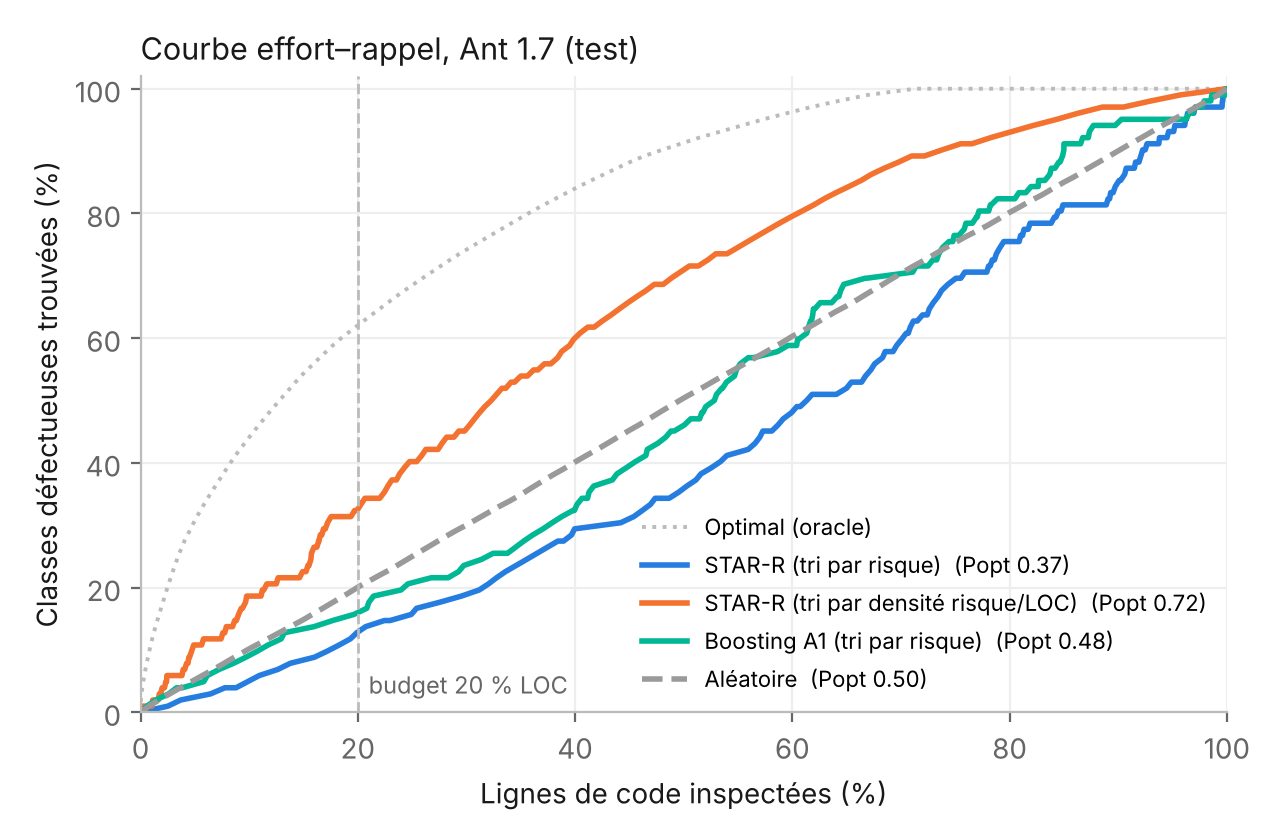
\includegraphics[width=0.86\linewidth]{figures/budget_recall.png}
\caption{Courbe effort--rappel sur Ant 1.7. $P_{\mathrm{opt}}$ : aire normalisée (1 = oracle, $\approx$0,5 = hasard).}
\label{fig:budget}
\end{figure}

\begin{table}[htbp]
\centering\small
\caption{Part des classes défectueuses trouvées selon le budget en lignes de code (Ant 1.7).}
\label{tab:budget}
\rowcolors{2}{}{lightbg}
\begin{tabular}{lccccc}
\toprule
\textbf{Ordre d'inspection} & \textbf{10\,\%} & \textbf{20\,\%} & \textbf{30\,\%} & \textbf{50\,\%} & $\boldsymbol{P_{\mathrm{opt}}}$ \\
\midrule
STAR-R, tri par risque brut           & 0,05 & 0,13 & 0,19 & 0,36 & 0,37 \\
STAR-R, tri par densité risque/LOC    & \best{0,19} & \best{0,33} & \best{0,45} & \best{0,71} & \best{0,72} \\
Boosting A1, tri par risque brut      & 0,09 & 0,16 & 0,24 & 0,46 & 0,48 \\
Inspection aléatoire                  & 0,10 & 0,20 & 0,30 & 0,50 & 0,50 \\
\bottomrule
\end{tabular}
\end{table}

\begin{warnbox}[Résultat important]
Trié par risque brut, le modèle fait \emph{moins bien que le hasard} à budget de lignes de code fixé. Les classes
défectueuses sont en effet beaucoup plus grandes (médiane de 517 LOC contre 104 pour les saines) : le modèle les
détecte bien, mais les inspecter d'abord épuise le budget. Trier par \textbf{densité de risque} (score/LOC) corrige
ce biais sans modifier le modèle, et trouve 2,5 fois plus de défauts à 20\,\% des LOC (0,33 contre 0,13).
\end{warnbox}

\section{Poids de fusion et accord entre les vues}
\label{sec:fusion}
\begin{figure}[htbp]
\centering
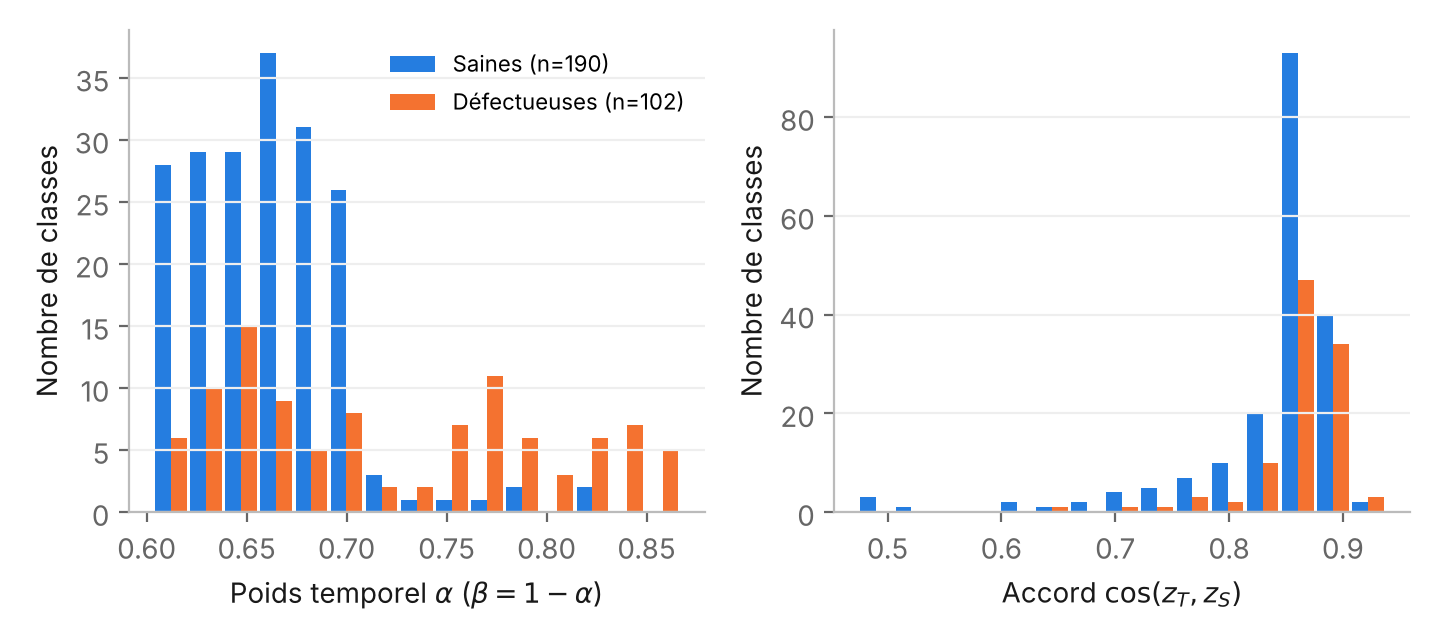
\includegraphics[width=0.9\linewidth]{figures/fusion_weights.png}
\caption{Distribution du poids temporel $\alpha$ (gauche) et de l'accord $\cos(z_T,z_S)$ (droite) selon le label,
sur Ant 1.7 (moyenne des 10 réseaux).}
\label{fig:fusion}
\end{figure}

\begin{itemize}
  \item \textbf{La vue temporelle domine} : $\alpha$ est compris entre 0,59 et 0,87 pour toutes les classes. Le modèle
        s'appuie surtout sur l'historique des métriques.
  \item \textbf{$\alpha$ est plus élevé pour les classes défectueuses} : 0,72 en moyenne contre 0,66 pour les saines,
        et parmi les classes où $\alpha>0{,}72$, 47 sur 54 sont défectueuses. Pour les classes à risque, le modèle donne
        encore plus de poids à l'historique.
  \item \textbf{L'accord cosinus discrimine peu} : 0,86 en moyenne pour les défectueuses contre 0,84 pour les saines.
        Les deux vues sont fortement alignées (effet de l'InfoNCE), si bien que l'accord porte peu d'information propre.
        Cela explique pourquoi la fusion guidée (A4) apporte peu par rapport à la fusion classique (A3).
  \item Avec la régularisation par l'entropie de la porte (G2, section~\ref{sec:improve}), le poids temporel moyen
        descend à 0,55 sans perte de performance : la domination de la vue temporelle n'est donc pas nécessaire à la
        qualité du classement.
\end{itemize}

\section{Analyse des erreurs}
Avec le seuil choisi sur la validation, le modèle signale comme défectueuses les 96 classes les plus risquées
(33\,\% des classes). Le tableau~\ref{tab:confusion} résume le résultat.

\begin{table}[H]
\centering\small
\caption{Matrice de confusion sur Ant 1.7 (292 classes, seuil de 96 classes signalées).}
\label{tab:confusion}
\begin{tabular}{lcc}
\toprule
 & \textbf{Défectueuse en réalité} & \textbf{Saine en réalité} \\
\midrule
\textbf{Signalée par le modèle} & 73 (vrais positifs) & 23 (faux positifs) \\
\textbf{Non signalée}           & 29 (défauts manqués) & 167 (vrais négatifs) \\
\bottomrule
\end{tabular}
\end{table}

Le modèle retrouve 73 des 102 classes défectueuses (rappel de 72\,\%), et 76\,\% des classes qu'il signale sont
réellement défectueuses. Pour comprendre les 52 erreurs, le tableau~\ref{tab:errors} présente les cas les plus
marqués : les classes saines jugées les plus risquées, et les classes défectueuses jugées les moins risquées.
Pour comparaison, la classe médiane du projet compte 164 lignes de code, un WMC de 8, un CBO de 8 et un RFC de 25.

\begin{table}[H]
\centering\small
\caption{Erreurs typiques sur Ant 1.7 (préfixe \code{org.apache.tools.ant} omis). Rang : position dans le tri par
risque brut, sur 292.}
\label{tab:errors}
\begin{tabular}{rlrrrr}
\toprule
\textbf{Rang} & \textbf{Classe} & \textbf{LOC} & \textbf{WMC} & \textbf{CBO} & \textbf{RFC} \\
\midrule
\multicolumn{6}{l}{\textit{Faux positifs les mieux classés (saines mais jugées très risquées)}} \\
5  & \code{taskdefs.Execute}         & 1095 & 33 & 70 & 121 \\
17 & \code{taskdefs.ExecuteJava}     & 552  & 13 & 24 & 82 \\
31 & \code{types.CommandlineJava}    & 559  & 39 & 21 & 94 \\
39 & \code{types.XMLCatalog}         & 874  & 28 & 17 & 105 \\
\midrule
\multicolumn{6}{l}{\textit{Défauts manqués les plus mal classés (défectueuses mais jugées peu risquées)}} \\
201 & \code{util.Watchdog}            & 112 & 7 & 3  & 22 \\
254 & \code{types.Substitution}       & 33  & 4 & 5  & 7 \\
257 & \code{NoBannerLogger}           & 57  & 4 & 4  & 17 \\
264 & \code{BuildListener}            & 7   & 7 & 16 & 7 \\
\bottomrule
\end{tabular}
\end{table}

\subsection{Faux positifs : des classes grandes et très couplées}
Les quatre faux positifs les mieux classés ont entre 3 et 7 fois plus de lignes de code que la classe médiane, et
un RFC 3 à 5 fois plus élevé. \code{taskdefs.Execute} en est l'exemple extrême : 1\,095 lignes et un couplage
(CBO) de 70, presque 9 fois la médiane. Ce sont exactement les caractéristiques qui accompagnent le plus souvent un
défaut dans les données d'entraînement ; le modèle a donc appris une règle juste en moyenne, mais qui se trompe sur
les grandes classes bien testées.

\subsection{Défauts manqués : des petites classes aux métriques banales}
À l'inverse, les défauts les plus mal classés touchent de petites classes simples : de 7 à 130 lignes, avec un WMC
de 4 à 7, sous la médiane du projet. \code{BuildListener} n'a que 7 lignes : c'est une interface, dont le défaut
vient probablement d'un changement de contrat qui se propage aux classes qui l'implémentent, et non de sa
complexité interne. Son CBO de 16, le double de la médiane, est le seul signal, mais il ne suffit pas face à sa
taille minuscule. Pour ces classes, rien dans les 20 métriques ne distingue une classe défectueuse d'une classe
saine.

\subsection{Ce que ces erreurs apprennent}
\begin{itemize}
  \item \textbf{Le modèle confond en partie « grand et complexe » et « défectueux ».} Les faux positifs ont une
        médiane de 377 lignes, les défauts manqués de 182 lignes. Le modèle ne
        voit que la structure du code : un défaut sans trace dans ces métriques lui reste invisible.
  \item \textbf{Le tri par densité corrige une partie de ces erreurs.} En divisant le score par le nombre de lignes,
        \code{taskdefs.Execute} recule de la 5\textsuperscript{e} à la 262\textsuperscript{e} place, tandis que
        \code{BuildListener} remonte de la 264\textsuperscript{e} à la 26\textsuperscript{e} et \code{types.Substitution}
        de la 254\textsuperscript{e} à la 74\textsuperscript{e}. C'est la raison pour laquelle cet ordre trouve 2,5 fois
        plus de défauts à budget égal (tableau~\ref{tab:budget}).
  \item \textbf{Piste d'amélioration.} Les défauts des petites classes dépendent surtout de l'historique des
        modifications (nombre de commits, nombre de développeurs, changements récents) plutôt que de leur structure.
        Ajouter ces métriques de processus~\cite{moser2008} est la piste la plus prometteuse pour les détecter.
\end{itemize}


\section{Pourquoi le graphe aide sur Camel}
\label{sec:graph}
Le script \code{graph\_analysis.py} mesure, sur la version de test de chaque projet, la structure du graphe d'imports et
l'apport du graphe (A3 contre A2, réglages d'Ant, 5 graines) séparément pour les classes isolées (aucun import entrant
ni sortant) et connectées. Les labels ne servent qu'à l'évaluation.

\begin{table}[H]
\centering\small
\caption{Graphe d'imports et apport du graphe selon la connectivité (version de test).}
\label{tab:graph}
\rowcolors{2}{}{lightbg}
\begin{tabularx}{\linewidth}{>{\raggedright\arraybackslash}Xccc}
\toprule
 & \textbf{Ant 1.7} & \textbf{Camel 1.6} & \textbf{POI 3.0} \\
\midrule
Classes isolées                                   & 12,7\,\% & 14,2\,\% & 25,4\,\% \\
\% défectueuses : isolées $\to$ connectées & 21,6 $\to$ 36,9 ($\times$1,7) & \best{1,3 $\to$ 26,0 ($\times$20)} & 55,7 $\to$ 68,1 ($\times$1,2) \\
Homophilie (voisins défectueux : déf.\ $-$ saines) & $+0{,}03$ & $-0{,}01$ & $+0{,}12$ \\
Apport du graphe, classes connectées ($\Delta$AP) & $+0{,}001$ & \best{$+0{,}052$} & $-0{,}152$ \\
Apport du graphe, classes isolées ($\Delta$AP)    & $+0{,}005$ & $-0{,}001$ & $-0{,}000$ \\
\bottomrule
\end{tabularx}
\end{table}

Sur Camel, une classe isolée n'est presque jamais défectueuse (1 sur 80), et tout le gain du graphe porte sur les
classes connectées. Les classes défectueuses ne s'importent pas davantage entre elles (homophilie nulle) : le signal est
la \emph{connectivité} elle-même, que l'agrégation de GraphSAGE capte et que les métriques de couplage (CBO, Ca, Ce) ne
reflètent qu'en partie. Sur Ant, ce contraste est faible ($\times$1,7) et le graphe n'ajoute rien. Sur POI, le graphe
dégrade les résultats malgré la plus forte homophilie : la cause la plus probable est le transfert des réglages d'Ant.
Avec trois projets informatifs, il s'agit d'une explication corrélationnelle, non d'une preuve.

% ============================================================ 7. Application
\chapter{Application de visualisation}

L'application \code{app.py} (Streamlit) présente la liste priorisée produite par le modèle final
(figure~\ref{fig:app}). Elle permet de :
\begin{itemize}
  \item choisir l'ordre d'inspection : densité de risque (recommandé) ou risque brut ;
  \item fixer un budget, en pourcentage des lignes de code ou en nombre de classes (Top-$k$) ;
  \item voir les classes à inspecter avec leur score, leur risque par kLOC, leurs métriques et leurs poids de fusion ;
  \item afficher, en mode évaluation, les défauts réellement trouvés, le rappel et la précision du budget choisi ;
  \item consulter le détail d'une classe en comparant ses métriques à la médiane du projet ;
  \item suivre la courbe effort--rappel interactive et télécharger la sélection au format CSV.
\end{itemize}

\begin{figure}[htbp]
\centering
\fcolorbox{rulegray}{white}{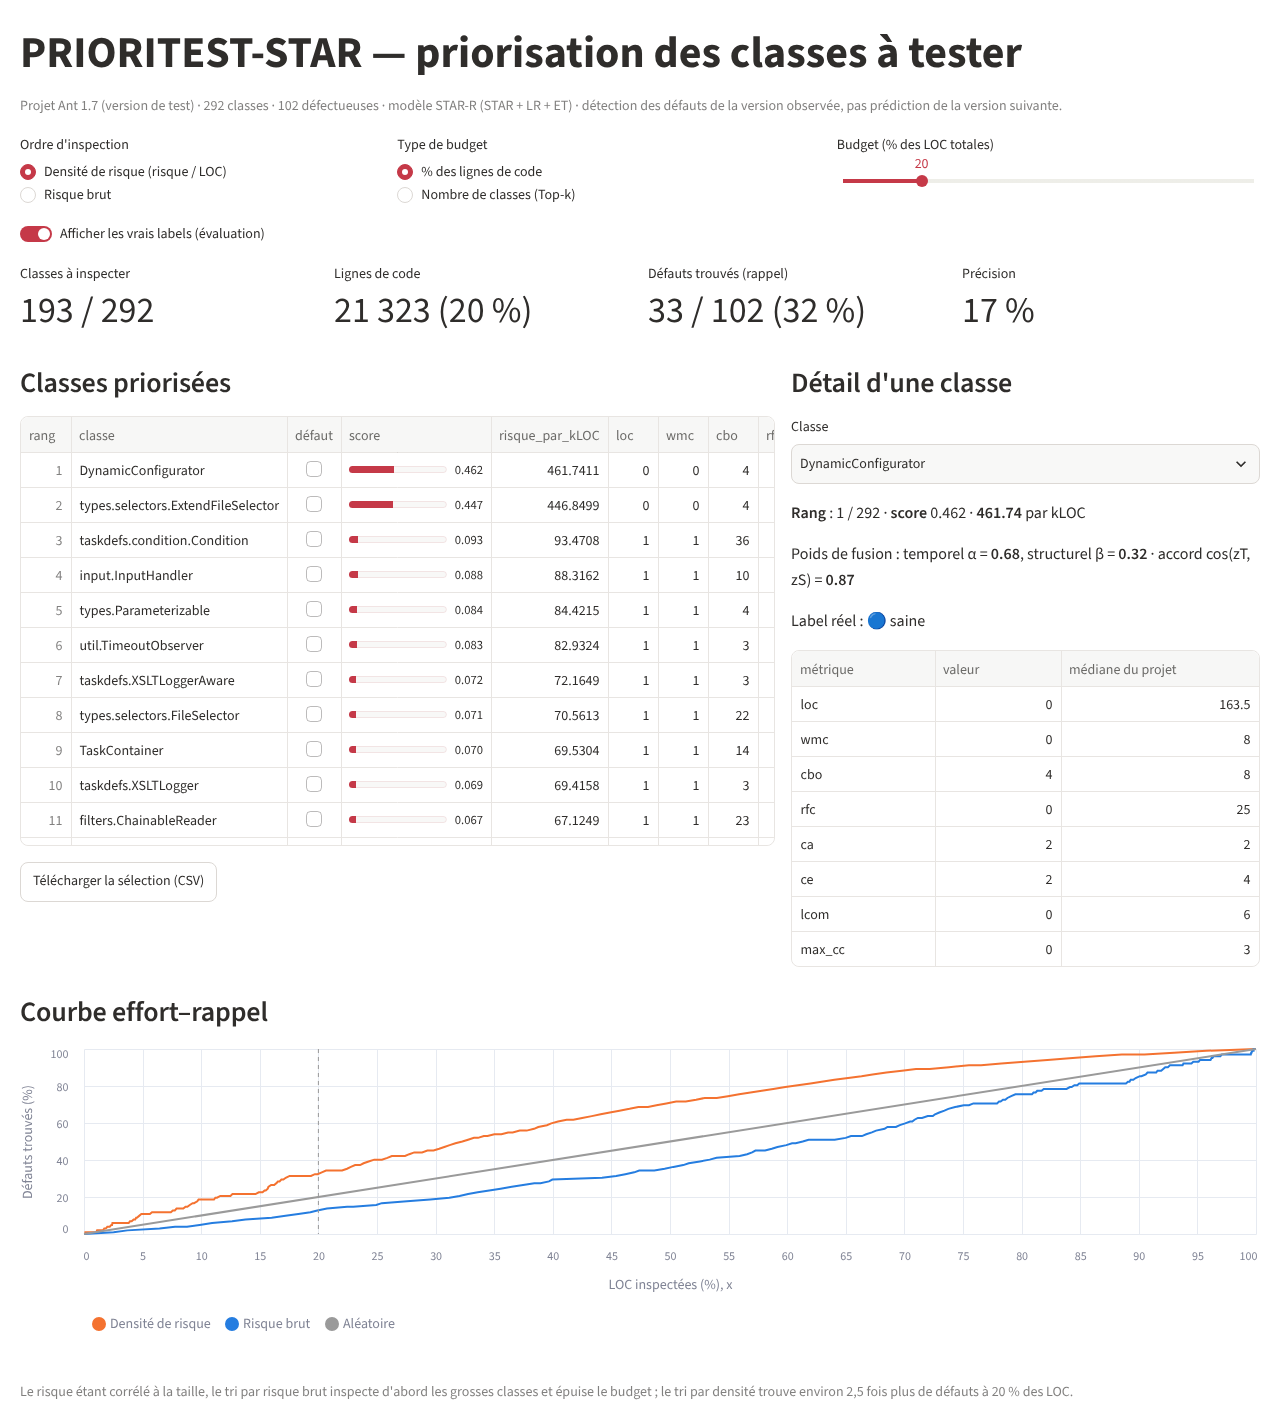
\includegraphics[width=0.92\linewidth]{figures/app_screenshot.png}}
\caption{Application de visualisation : budget de 20\,\% des LOC, tri par densité de risque.}
\label{fig:app}
\end{figure}

\section{Reproduction}
\label{sec:repro}
\begin{tcolorbox}[colback=lightbg,colframe=rulegray,boxrule=0.5pt,arc=2pt,left=6pt]
\small
\begin{verbatim}
pip install -r requirements.txt
python -m unittest discover -s tests -v
python run_star.py --project ant --seeds 42 43 44 45 46
python explore_val.py --project ant
python train_final.py --project ant --groups 5 --ens 10
python analyse_star.py --project ant
python compare_fair.py --project ant        # sec. 5.4 (~6,5 min)
python effort_star.py --project ant         # sec. 5.5 (~4 min)
python more_data.py --project ant           # sec. 5.6 (~4 min)
python improve_star.py --project ant        # sec. 5.7 (~5 min)
python transfer_study.py                    # sec. 5.8 (~5 min)
python retune_project.py --projects camel   # sec. 5.8 (~6 min)
python graph_analysis.py                    # sec. 6.4 (15 s)
streamlit run app.py
\end{verbatim}
\end{tcolorbox}

% ============================================================ 8. Conclusion
\chapter{Conclusion et perspectives}

\section{Bilan}
Nous avons étudié, audité et amélioré PRIORITEST-STAR, un modèle à deux vues (TCN sur l'historique, GraphSAGE sur
les imports) avec fusion guidée par similarité, InfoNCE inter-vues et RankNet. Le protocole est chronologique et sans
fuite. La procédure STAR-R réduit fortement la variance et atteint sur Ant 1.7 une AP de 0,799, une accuracy de
0,823 et un F1 de 0,745.

En réponse à la question de recherche, la réponse est \textbf{nuancée et dépend du projet} :
\begin{itemize}
  \item \textbf{Sur Ant}, à réglage égal, la fusion guidée et l'alignement contrastif ne sont pas supérieurs à une
        référence tabulaire bien réglée ; aucun mécanisme n'a d'effet significatif, et l'accord entre les vues
        discrimine peu.
  \item \textbf{Sur Camel}, réglé sur ses propres données, STAR avec le graphe dépasse la régression logistique
        d'environ $+0{,}09$ d'AP ($p\le0{,}01$). Le graphe y apporte un signal de connectivité que les métriques ne
        contiennent pas.
  \item \textbf{STAR exploite mieux qu'un modèle linéaire les données d'autres projets} (Ant, POI, tendance sur Camel),
        et le mélange STAR + LR + ET améliore le classement sensible à l'effort sur Ant et Camel.
  \item \textbf{RankNet dégrade les résultats} sur Ant comme sur Camel, et intégrer l'effort dans la perte (STAR-E)
        n'apporte rien de plus que le tri par densité.
\end{itemize}
L'ordre d'inspection compte beaucoup : trier par densité de risque multiplie par 2,5 les défauts trouvés à budget égal
sur Ant. Les modèles à base d'arbres (Random Forest, ExtraTrees) restent les références sensibles à l'effort les plus
sûres.

\section{Limites}
\begin{itemize}
  \item Un seul projet (Ant) dispose de trois fenêtres exploitables, avec 118 classes d'entraînement ; Camel et POI
        n'ont pas de version de validation indépendante, et JEdit 4.3 ne contient que 5 défauts.
  \item Une seule version de test par projet : avec quelques centaines de classes, les intervalles de confiance de
        l'AP sont larges (environ $\pm0{,}07$ à $\pm0{,}09$).
  \item Classes nouvelles exclues, d'où un biais de sélection ; leurs labels ne figurent pas dans le kit. Graphe
        d'imports partiel.
  \item Les mêmes classes apparaissent à l'entraînement et au test, à des versions différentes.
  \item Détection des défauts de la version courante, et non prédiction prospective.
\end{itemize}

\section{Perspectives}
\begin{itemize}
  \item Terminer le réglage interne sur POI et classer tous les modèles par la méthode de Scott-Knott ESD, déjà
        implémentée.
  \item Adaptation de domaine pour tirer parti des données d'autres projets (normalisation par projet apprise,
        pondération des projets sources selon leur ressemblance avec le projet cible).
  \item GNN temporel sur le graphe multi-versions déjà fourni (\code{\_graph\_temporal.npz}) et étude des classes
        nouvelles, à partir de l'archive PROMISE complète.
  \item Ajout de métriques de processus (nombre de modifications, auteurs) pour mieux détecter les petites classes
        défectueuses.
  \item Protocole réellement prospectif ($t\to t+1$), après vérification de la disponibilité des labels.
\end{itemize}

% ============================================================ Bibliographie
\begin{thebibliography}{99}
\small
\bibitem{ck1994} S.~R. Chidamber and C.~F. Kemerer, ``A metrics suite for object oriented design,''
  \emph{IEEE Transactions on Software Engineering}, 20(6):476--493, 1994.
\bibitem{basili1996} V.~R. Basili, L.~C. Briand and W.~L. Melo, ``A validation of object-oriented design metrics as
  quality indicators,'' \emph{IEEE Transactions on Software Engineering}, 22(10):751--761, 1996.
\bibitem{jureczko2010} M.~Jureczko and L.~Madeyski, ``Towards identifying software project clusters with regard to
  defect prediction,'' in \emph{Proc. PROMISE}, 2010.
\bibitem{menzies2007} T.~Menzies, J.~Greenwald and A.~Frank, ``Data mining static code attributes to learn defect
  predictors,'' \emph{IEEE Transactions on Software Engineering}, 33(1):2--13, 2007.
\bibitem{lessmann2008} S.~Lessmann, B.~Baesens, C.~Mues and S.~Pietsch, ``Benchmarking classification models for
  software defect prediction: A proposed framework and novel findings,'' \emph{IEEE Transactions on Software
  Engineering}, 34(4):485--496, 2008.
\bibitem{ghotra2015} B.~Ghotra, S.~McIntosh and A.~E. Hassan, ``Revisiting the impact of classification techniques
  on the performance of defect prediction models,'' in \emph{Proc. ICSE}, 2015.
\bibitem{tantithamthavorn2016} C.~Tantithamthavorn, S.~McIntosh, A.~E. Hassan and K.~Matsumoto, ``Automated parameter
  optimization of classification techniques for defect prediction models,'' in \emph{Proc. ICSE}, 2016.
\bibitem{moser2008} R.~Moser, W.~Pedrycz and G.~Succi, ``A comparative analysis of the efficiency of change metrics
  and static code attributes for defect prediction,'' in \emph{Proc. ICSE}, 2008.
\bibitem{wang2016} S.~Wang, T.~Liu and L.~Tan, ``Automatically learning semantic features for defect prediction,''
  in \emph{Proc. ICSE}, 2016.
\bibitem{li2017} J.~Li, P.~He, J.~Zhu and M.~R. Lyu, ``Software defect prediction via convolutional neural network,''
  in \emph{Proc. QRS}, 2017.
\bibitem{rhazi2026} A.-R. Rhazi, O.~Banouar, F.~Toure and S.~Raghay, ``Software defect prediction via contrastive
  similarity learning and inter-sample attention,'' \emph{Science of Computer Programming}, 254:103534, 2026.
  doi:10.1016/j.scico.2026.103534.
\bibitem{zimmermann2008} T.~Zimmermann and N.~Nagappan, ``Predicting defects using network analysis on dependency
  graphs,'' in \emph{Proc. ICSE}, 2008.
\bibitem{hamilton2017} W.~L. Hamilton, R.~Ying and J.~Leskovec, ``Inductive representation learning on large
  graphs,'' in \emph{Proc. NeurIPS}, 2017.
\bibitem{bai2018} S.~Bai, J.~Z. Kolter and V.~Koltun, ``An empirical evaluation of generic convolutional and
  recurrent networks for sequence modeling,'' arXiv:1803.01271, 2018.
\bibitem{oord2018} A.~van den Oord, Y.~Li and O.~Vinyals, ``Representation learning with contrastive predictive
  coding,'' arXiv:1807.03748, 2018.
\bibitem{chen2020} T.~Chen, S.~Kornblith, M.~Norouzi and G.~Hinton, ``A simple framework for contrastive learning of
  visual representations,'' in \emph{Proc. ICML}, 2020.
\bibitem{khosla2020} P.~Khosla et al., ``Supervised contrastive learning,'' in \emph{Proc. NeurIPS}, 2020.
\bibitem{burges2005} C.~Burges et al., ``Learning to rank using gradient descent,'' in \emph{Proc. ICML}, 2005.
\bibitem{mende2010} T.~Mende and R.~Koschke, ``Effort-aware defect prediction models,'' in \emph{Proc. CSMR}, 2010.
\bibitem{kamei2013} Y.~Kamei et al., ``A large-scale empirical study of just-in-time quality assurance,''
  \emph{IEEE Transactions on Software Engineering}, 39(6):757--773, 2013.
\bibitem{yang2016} Y.~Yang et al., ``Effort-aware just-in-time defect prediction: Simple unsupervised models could be
  better than supervised models,'' in \emph{Proc. FSE}, 2016.
\bibitem{efron1993} B.~Efron and R.~J. Tibshirani, \emph{An Introduction to the Bootstrap}, Chapman \& Hall, 1993.
\bibitem{wilcoxon1945} F.~Wilcoxon, ``Individual comparisons by ranking methods,'' \emph{Biometrics Bulletin},
  1(6):80--83, 1945.
\bibitem{romano2006} J.~Romano, J.~D. Kromrey, J.~Coraggio and J.~Skowronek, ``Appropriate statistics for ordinal
  level data: Should we really be using t-test and Cohen's d for evaluating group differences on the NSSE and other
  surveys?,'' in \emph{Annual Meeting of the Florida Association of Institutional Research}, 2006.
\end{thebibliography}

\end{document}
